\section{Pre-Registered Decision Criteria (Verbatim Summary)}
\label{app:prereg}

The following criteria were fixed in \texttt{experiment\_design.md} before any paid GPU run, after two rounds of external automated review (one at design v1, one at v2/v3). Let $m=\log 1.25$ on the log primary outcome.

\begin{itemize}
\item \textbf{Regularizer fixes drift:} $C_R$ CI excludes 0 in the improving direction on $\geq 2$ of 3 dynamics families (the two point-mass environments count as one family), and the P0+R2 vs.\ P1 contrast CI lies entirely inside $[-m,m]$ (TOST-style equivalence), without collapse.
\item \textbf{Protocol dominates:} $C_P$ CI excludes 0 in $\geq 2$ of 3 families AND $C_R$ equivalence-to-zero holds.
\item \textbf{Interaction:} $C_I$ CI excludes 0 in $\geq 2$ families, or a CI-supported sign flip of $C_R$ between protocols.
\item \textbf{Encoder geometry:} in the swap $2{\times}2$, the primary outcome follows encoder source rather than dynamics-retraining protocol (interaction-contrast CI).
\item \textbf{Null/equivalence:} $C_R$, $C_P$, $C_I$ CIs all inside $[-m,m]$.
\item \textbf{Mixed:} anything else, reported as such with all contrast CIs.
\end{itemize}

Outcome: $C_R$, $C_P$, and $C_I$ were censored by differential collapse (no surviving R0 cell exists anywhere in the design); the realized verdict is \textbf{mixed}, with the conditional protocol contrasts $C_{P\mid R1}$, $C_{P\mid R2}$ supported on Lorenz. The collapse rule and the collapse-as-outcome analysis were themselves pre-registered, which is why the censoring is reportable rather than fatal.

\section{Deviation Ledger}
\label{app:deviations}

All deviations from the pre-registered design, with causes. Items 1--5 were forced by an 8-hour wall-clock constraint imposed mid-execution; items 6--8 were discovered in post-hoc code audit.

\begin{enumerate}
\item \textbf{Training steps reduced uniformly}: state $20\text{k}\!\to\!10\text{k}$, visual $15\text{k}\!\to\!8\text{k}$, identically for every condition. Uniform in treatment but not necessarily treatment-neutral (conditions may converge at different rates); all claims hold at the observed training horizon.
\item \textbf{Visual seeds} $5\to3$ (reverting to the original scope).
\item \textbf{Dropped arms}: $\lambda$-sensitivity (24 runs), matched latent dimension (24), $M{=}1024$ projections (2), rollout-regularization ablation (12). The $\lambda$-sensitivity drop is the most consequential (Section~5, Limitation 1).
\item \textbf{Encoder-swap restructured}: phase-A source models were taken from checkpointed core-sweep cells rather than trained separately (saving 12 runs); the $2{\times}2$ retains retrained diagonals.
\item \textbf{$\lambda$-pilot steps} reduced to 8k/4k (state/visual); pilots rank candidates, and all candidates within a cell share the budget.
\item \textbf{Validation split used for final metrics} instead of the generated test split (pre-registration specified test).
\item \textbf{Evaluation windows sampled per run} rather than from a fixed shared evaluation suite, weakening seed-pairing across conditions.
\item \textbf{Shared RNG stream}: the regularizer's random projections consume the same generator as minibatch sampling, so R2 conditions saw different minibatch sequences than R0/R1 at equal seed.
\item \textbf{SIGReg parity test not executed}: the pre-registered loss/gradient parity check against the official LeWorldModel implementation was specified but not run before the sweep; R2 claims are implementation-specific (exact-integral EP variant).
\end{enumerate}

\section{Weight-Selection Audit}
\label{app:lambda}

\begin{figure}[h]
  \centering
  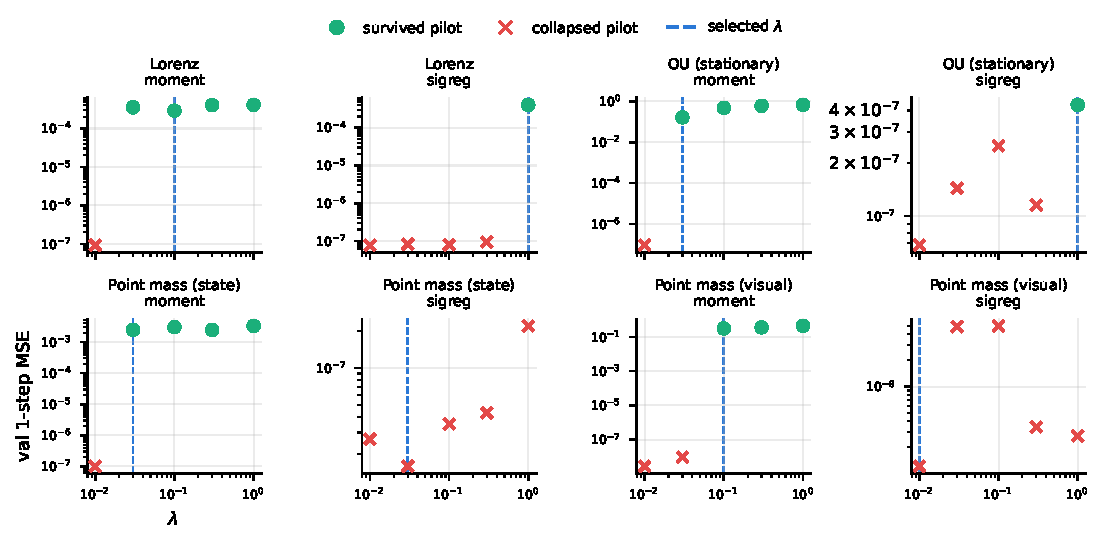
\includegraphics[width=\linewidth]{figures/fig7_lambda_frontier.pdf}
  \caption{The full $\lambda$-pilot grid (seed 0, 1-step protocol, reduced pilot budget): validation one-step MSE versus $\lambda$, colored by the pilot collapse screen. Collapsed pilots exhibit spuriously tiny validation MSE ($10^{-9}$--$10^{-7}$), which is why validation error alone cannot be trusted for weight selection. For EP-SIGReg on OU and Lorenz only the grid boundary $\lambda{=}1.0$ survived the screen; on both point-mass environments no grid point survived and the pre-registered fallback (best validation MSE among all candidates) then actively favored the most degenerate solution.}
  \label{fig:lambda}
\end{figure}

Table~\ref{tab:lambda} lists selections. Three structural observations: (i) at low $\lambda$ every regularizer collapses, as expected, since R0 always collapses; (ii) for EP-SIGReg the surviving region is empty (point mass) or a boundary point (OU, Lorenz); (iii) the OU boundary survivor at pilot length ($8$k steps, val MSE $4.3\times10^{-7}$, probe $R^2$ 0.89) slid into dimensional collapse at full length ($10$k steps) in 10/10 main runs, i.e.\ the pilot screen passed a configuration that was already en route to the collapsed stationary point.

\begin{table}[h]
\centering
\caption{Selected $\lambda$ per (regularizer, environment). ``All collapsed'' marks cells where no grid point passed the pilot collapse screen and the fallback selected on validation MSE alone.}
\label{tab:lambda}
\small
\begin{tabular}{llcc}
\toprule
Environment & Regularizer & Selected $\lambda$ & Pilot grid status \\
\midrule
Stable linear (det.) & moment & 0.01 & all 5 survived \\
OU & moment & 0.03 & 4/5 survived \\
OU & EP-SIGReg & 1.0 & only boundary survived \\
Lorenz & moment & 0.1 & 4/5 survived \\
Lorenz & EP-SIGReg & 1.0 & only boundary survived \\
Point mass (state) & moment & 0.03 & 4/5 survived \\
Point mass (state) & EP-SIGReg & 0.03 & \textbf{all collapsed} \\
Point mass (visual) & moment & 0.1 & 3/5 survived \\
Point mass (visual) & EP-SIGReg & 0.01 & \textbf{all collapsed} \\
\bottomrule
\end{tabular}
\end{table}

The R1 and R2 loss scales also differ substantially (the EP statistic is bounded; the moment penalty is not), so the shared numerical grid is not dose-matched between regularizers; between-regularizer collapse comparisons should be read with that in mind.

\section{The Collapsed Stationary Point of the Epps--Pulley Loss}
\label{app:stationary}

Let all latents be identical, $Z\equiv c$ for a constant $c\in\mathbb{R}^d$ (variance collapse; $c=0$ after any centering). Every projection is then the constant $h_i\equiv h_0=\langle c,u\rangle$. Substituting into Eq.~(1) of the main text:
\begin{align}
\mathrm{EP}_\gamma(h) &= \frac{1}{B^2}\sum_{i,j} e^{-\gamma(h_0-h_0)^2} + \frac{1}{\sqrt{1+4\gamma}} - \frac{2}{\sqrt{1+2\gamma}}\, e^{-\gamma h_0^2/(1+2\gamma)} \nonumber\\
&= 1 + \frac{1}{\sqrt{1+4\gamma}} - \frac{2}{\sqrt{1+2\gamma}}\, e^{-\gamma h_0^2/(1+2\gamma)}.
\end{align}
At $h_0=0$ and $\gamma=\nicefrac12$ this is $1+\nicefrac{1}{\sqrt3}-\sqrt2\approx 0.16308$. The sample--sample term is constant in $Z$ on the collapsed manifold and the sample--prior term is maximized at $h_0=0$, so $Z\equiv0$ is a stationary point of $\mathrm{EP}_\gamma$ (by symmetry of the Gaussian weighting, the gradient vanishes there), and because the statistic is an MMD it is \emph{bounded}: the penalty for total collapse saturates at $\approx0.163$ per projection. The empirical check: across the 33 collapsed EP-SIGReg runs in the main factorial, the median final regularizer loss is $0.1631$ (range $0.103$--$0.163$), matching the theoretical value to four digits, and 19/33 of those runs are variance collapses.

Contrast the moment proxy at the same point: $\lVert\mu\rVert^2+\lVert 0 - I\rVert_F^2 = \lVert c\rVert^2 + d$, which is at least $d=16$, two orders of magnitude larger, and grows with latent dimension. A trajectory approaching total collapse therefore feels a vanishing restoring force from the EP penalty but a large one from the moment penalty. We offer this as a candidate optimization-level explanation of the differential collapse pattern, consistent with the logged losses; establishing causality would require intervention (e.g., penalties modified to diverge at degeneracy, or warm starts displaced from the stationary point), which we leave to follow-up work.

Note the interplay with prediction: at $Z\equiv0$ the one-step prediction loss is also globally minimal (the dynamics maps $0\mapsto0$), so the collapsed configuration is a joint stationary point of the \emph{total} objective in which validation one-step MSE looks excellent. This is why the failure is invisible, indeed attractive, to validation-error-based model selection, and why the pilot screen's diagnostics (effective dimension, rank, probe $R^2$) are the only part of the selection protocol that resists it.

\section{Additional Results}
\label{app:extra}

\subsection{Collapse-Mode Decomposition}

Across all 144 factorial/control runs: 58 viable, 48 variance collapses, 8 dimensional, 30 informational. By regularizer (collapsed runs only): R0, 29 variance / 0 dimensional / 17 informational of 46; R1, 0/3/4 of 7; R2, 19/5/9 of 33. Figure~\ref{fig:effdim} shows the two collapse axes are genuinely distinct: a band of runs with effective dimension $<2$ retains probe $R^2>0.65$.

\begin{figure}[h]
  \centering
  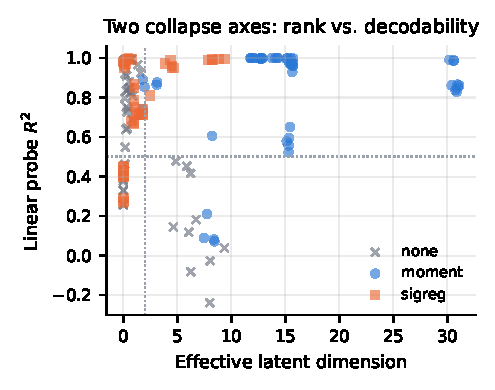
\includegraphics[width=0.55\linewidth]{figures/fig6_effdim_probe.pdf}
  \caption{Effective latent dimension versus linear-probe $R^2$, one point per run. Dotted lines mark the collapse thresholds. Rank-deficient codes (left of the vertical line) frequently remain decodable (above the horizontal line), which is why we report variance, dimensional, and informational collapse separately.}
  \label{fig:effdim}
\end{figure}

\subsection{Encoder-Swap $2{\times}2$}

\begin{figure}[h]
  \centering
  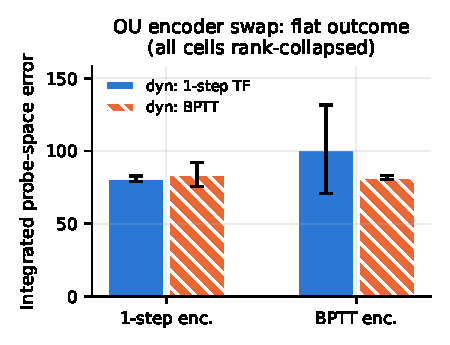
\includegraphics[width=0.5\linewidth]{figures/fig5_swap.pdf}
  \caption{Encoder-swap probe on OU (EP-SIGReg, seeds 0--2, retrained diagonals): integrated probe-space error is flat ($\approx80\pm5$) across all four encoder-source $\times$ dynamics-protocol cells; every cell is rank-collapsed and OU's rollout-error noise floor is $\approx76$. The probe is uninformative in this regime.}
  \label{fig:swap}
\end{figure}

\subsection{Lorenz Paired-Seed Detail}

Per-seed log effects of P1$-$P0 on the integrated primary outcome. Moment: $-1.84,-5.74,-2.70,-4.36,-0.80$ (mean $-3.09$; geometric ratio $0.046$; exact two-sided sign-flip $p=0.0625$; leave-one-out range $[-3.66,-2.42]$). EP-SIGReg: $-0.98,-2.17,-0.44,-0.70,-1.72$ (mean $-1.20$; ratio $0.30$; $p=0.0625$; LOO $[-1.39,-0.96]$). Exploratory regularizer contrast under P0 (R2$-$R1): mean $-1.82$ (ratio $0.162$, i.e.\ $6.2\times$ in R2's favor; $p=0.125$); under P1: $+0.06$ (ratio $1.07$; $p=0.56$). Horizon-resolved geometric ratios (P1/P0): moment $1.06,0.97,0.77,0.26,0.018$ and EP-SIGReg $2.63,2.08,1.29,0.34,0.16$ at $H=1,5,10,25,50$.

\subsection{Full Condition Summary}

\begin{table}[h]
\centering
\caption{All conditions: collapse probability and primary outcome conditional on survival (mean over surviving seeds; ``--'' = no survivors). Integrated probe-space open-loop error; lower is better; scales are environment-specific and not comparable across rows of different environments.}
\label{tab:full}
\small
\begin{tabular}{llccc}
\toprule
Environment & Reg. & Protocol & Collapse prob. & Primary $\mid$ viable \\
\midrule
Stable linear (det.) & none & P0 / P1 & 1.0 / 1.0 & -- / -- \\
Stable linear (det.) & moment & P0 / P1 & 0.0 / 0.8 & 2.99 / 2.68 \\
OU & none & P0 / P1 & 1.0 / 1.0 & -- / -- \\
OU & moment & P0 / P1 / P0.5 & 0.0 / 0.6 / 0.0 & 76.4 / 77.8 / 76.1 \\
OU & EP-SIGReg & P0 / P1 / P0.5 & 1.0 / 1.0 / 0.8 & -- / -- / 115.6 \\
Lorenz & none & P0 / P1 & 1.0 / 1.0 & -- / -- \\
Lorenz & moment & P0 / P1 & 0.0 / 0.0 & 9249 / 123 \\
Lorenz & EP-SIGReg & P0 / P1 & 0.0 / 0.0 & 573 / 134 \\
Point mass (state) & none & P0 / P1 & 1.0 / 1.0 & -- / -- \\
Point mass (state) & moment & P0 / P1 & 0.0 / 0.0 & 4.61 / 2.70 \\
Point mass (state) & EP-SIGReg & P0 / P1 & 1.0 / 1.0 & -- / -- \\
Point mass (visual) & none & P0 / P1 & 1.0 / 1.0 & -- / -- \\
Point mass (visual) & moment & P0 / P1 / P0.5 & 0.0 / 0.0 / 0.0 & 37.5 / 8.8 / 46.4 \\
Point mass (visual) & EP-SIGReg & P0 / P1 / P0.5 & 1.0 / 1.0 / 1.0 & -- / -- / -- \\
\bottomrule
\end{tabular}
\end{table}

\section{Compute Account}
\label{app:compute}

One RunPod instance, $7\times$ NVIDIA L4 24\,GB, 128 vCPUs. Total runs: 45 $\lambda$ pilots + 144 factorial/control + 12 swap = 201; zero failed jobs. A CPU-oversubscription pathology initially inflated per-step costs $\sim$$10\times$ (each PyTorch process spawned $\sim$35 threads; 7 concurrent jobs thrashed 128 vCPUs); capping \texttt{OMP\_NUM\_THREADS}=12 restored 96--98\% GPU utilization and roughly $3\times$ throughput. End-to-end wall clock from first pilot to finished analysis was under 3 hours against an 8-hour ceiling; total spend was under \$20 of a \$30 budget. Jobs were dispatched by a thread-safe GPU-pool runner (one job per GPU, round-robin) with stage-level hard-kill deadlines.

\section{Human--AI Session Flow and Division of Labor}
\label{app:session}

This study was conducted end-to-end by Claude (Anthropic; planning phases on Claude Fable 5, execution phases on Claude Sonnet 5) operating as an autonomous research agent under human direction, with OpenAI Codex (GPT-5-class, high reasoning effort) as an external automated reviewer at the design and results stages. The full machine-readable log is \texttt{session\_log.md} in the supplement. Summary of the division of labor:

\textbf{Human input.} (i) The research brief, verbatim: ``rollout drift in latent world models is caused by both the choice of marginal regularizer and the training protocol, and the two interact --- meaning neither can be studied in isolation [\dots] I don't want to specify what kinds of findings I'm looking for, because that would bias the experimental design. What I want from the results is honest engagement with the question --- experiments designed to distinguish between real possibilities rather than confirm a preferred answer.'' (ii) The compute budget (\$30 hard ceiling) and, mid-execution, an 8-hour wall-clock ceiling. (iii) Provisioning decisions: GPU vendor/type iterations (final: one $7\times$L4 instance) and SSH access. (iv) Approvals at phase boundaries; the instruction to proceed autonomously thereafter.

\textbf{AI work.} Literature positioning; adoption and revision of a prior interrupted session's design (v1) into v2--v4 under two external review rounds; all code (environments, regularizers, training protocols, metrics, sweep orchestration, GPU-pool runner, analysis); the $\lambda$ protocol; execution and monitoring on the remote instance; the mid-execution replan under the 8-hour constraint (uniform step reduction, arm drops, thread fix), logged before outcomes were seen; all statistical analysis including the post-review corrections (geometric effects, exact sign-flip tests, collapse-mode decomposition, stationary-point derivation and its empirical check); figures; and this manuscript.

\textbf{External automated review.} Codex review 1 (design stage) forced five major fixes before execution, including the stationary-Gaussian OU environment, the non-gameable primary metric, equalized regularizer exposure across protocols, contrast-based pre-registration with equivalence margins, and collapse-as-outcome analysis. Codex review 2 (results stage) corrected an arithmetic-mean effect size to its geometric value ($16\times\to6.2\times$), identified that the reported $C_P$ was actually $C_{P\mid R2}$, flagged the three pre-registration violations in the deviation ledger, proposed the collapse-mode decomposition and the $\lambda$-frontier audit, and contributed the observation that exact collapse is a stationary point of the EP loss with value $\approx0.163$, which we verified against the logged losses.

\textbf{Errors made and caught during the session} (retained for transparency): an initial GPU-dispatch bug that would have serialized all jobs onto one GPU (caught by utilization monitoring before damage); a stripped interpreter prefix that crashed all jobs instantly (caught within seconds); the CPU-thread oversubscription described in Appendix~\ref{app:compute} (caught by comparing isolated versus concurrent throughput); and an isolated-benchmark cost model that underestimated concurrent-load costs, corrected by re-benchmarking under realistic load before the main sweep.

\section{Reproducibility}
\label{app:repro}

The supplement contains: all source (\texttt{src/}), the pre-registration documents with full version history (\texttt{experiment\_design.md}, \texttt{compute\_budget.md} v1--v10), the session log, both external review transcripts, run manifests, per-run \texttt{metrics.json} for all 201 runs, the flat metrics table, and the analysis and figure scripts. Seeds: data generation, model init, and training are seeded per run (0--4); known seeding caveats are ledger items 7--8 of Appendix~\ref{app:deviations}.
